\chapter{Background}
\label{ch:background}

This chapter introduces some brief preliminary background that will be helpful for understanding \cref{ch:atrds}. Here, we will only introduce what is necessary, and not much more. However, we will cover some concepts in greater detail in \cref{app:atm}, \cref{app:risk}, and \cref{app:shrinkage}, at which point we will introduce further background as needed.

\section{Flight Delays and Weather}

The vast majority of flight delays and cancellations fall under three main categories, based on cause \cite{bts_causes_2024}:
\begin{enumerate}
    \item Carrier: resulting from circumstances within an airline's control, such as maintenance.
    \item NAS: a catch-all for anything from issues in the National Airspace System, such as non-extreme weather conditions and heavy traffic volume.
    \item Late aircraft: when an earlier flight that the present flight depended on arrived late.
\end{enumerate}

These reasons describe how flight delays can propagate through a larger network. Individual flights can accumulate delays through carrier and NAS delays, which are then passed on to later flights in the day through late aircraft delays, if the accumulated delays are sufficiently severe and the original schedule is sufficiently unforgiving. Later in \cref{ch:atrds}, we will focus on LGA for analysis, so we first take a brief look at its historical operations. In \cref{fig:delay-comparison}, this worsening of delays throughout the day is evident, and it also depicts a common response to worsening delays observed in the data from \cite{bts_transstats_nodate}, which is to begin canceling flights when the system cannot keep up with the scheduled demand while also trying to process delayed flights from earlier in the day. More such images may be found \href{here}{https://github.com/jz268/BayesAirATRDS2025/tree/main/scripts/notebooks/images}.

\begin{figure}[htb!]
    \centering
    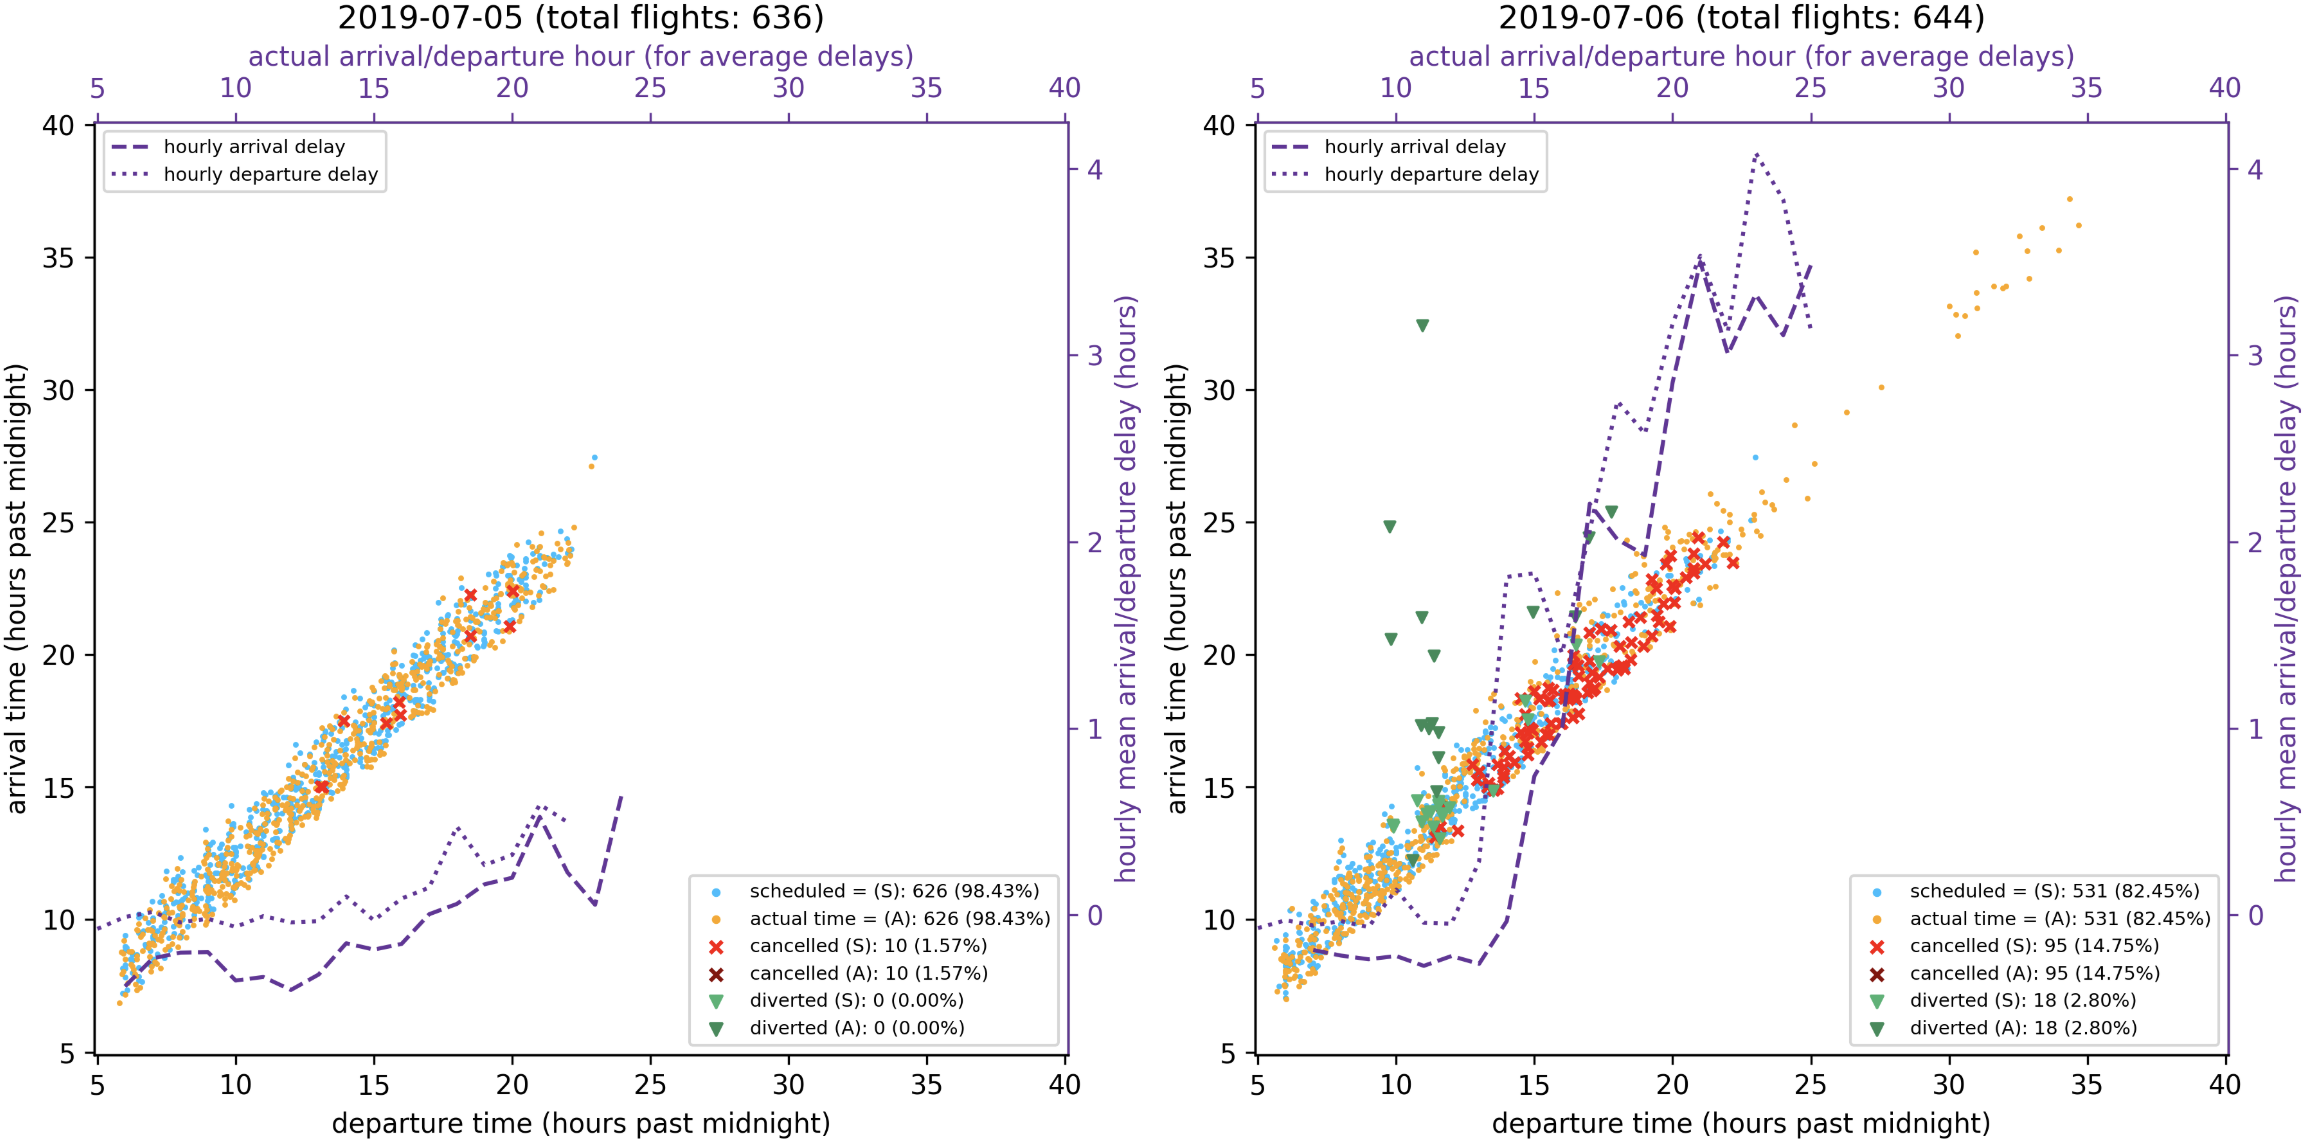
\includegraphics[width=\linewidth]{media/delay-comparison.png}
    \caption{Comparison of schedules and actual performance of flights at LGA in a day with significant delays and cancellations (right), and a day without (left). }
    \label{fig:delay-comparison}
\end{figure}

Other responses may be preemptive, in response to potential disruptions from weather events, implemented through Traffic Management Initiatives (TMI) \cite{jones_risk-adjusted_2023}. These often involve Traffic Flow Management System (TFMS) programs, which include ground delay programs (GDP), airspace flow programs (AFP), and collaborative trajectory options programs (CTOP). These programs can also have effects that span across the network, instead of just being localized at a single node. For example, in GDPs, aircraft are held on the ground at the origin airport of flights to help manage incoming demand at specific locations, eagerly shifting the delays to waiting on the ground rather than lazily accumulating flights in airborne holding, a less desirable position \cite{faa_tmi_2024}.

In particular, we can see the natural hierarchical structure to the problem, because the relationship between weather and delays is not always perfectly straightforward. However, the relationship between weather and certain intermediate factors, such as the aforementioned TMIs, and the relationship between those intermediate factors and observed delays, are more well-defined, and give us some structure work with.


\section{Posterior Approximation}
\label{background-approximate-inference}

In this and the following part, we will consider a simple model involving $\rx$ and $\rz$, where $\rx$ is observed and $\rz$ is a latent parameter. Given observations $x\in \Data$, we are often interested in inferring the posterior distribution of the latent parameters. Unfortunately, this posterior is often computationally intractable. To see why, suppose that we have $\pld{x\given z}$ as our model, and some prior $\pd{z}$. Then by applying Bayes' rule, we have
\begin{equation}
    \pld{z\given x} = \frac{\pld{x\given z}\pd{z}}{\pld{x}},
\end{equation}
where the marginal in the denominator is generally intractable as it requires computing
\begin{equation}
    \pld{x} = \int \pld{x\given z}\pd{z} \,dz.
\end{equation}
Instead, it is often more practical to approximate this posterior instead, using methods such as Laplace's approximation \cite{laplace1776}, or variational inference \cite{blei2017variational}, for example. In cases where the likelihoods aren't available either, there are other families of methods such as Markov Chain Monte Carlo (MCMC) \cite{metropolis_1953}, or Approximate Bayesian Computation (ABC) \cite{abc_2013} that can be used. We discuss these further in \cref{ch:lit-review}.


\section{Variational Inference}
\label{background-variational-inference}

We briefly introduce the concepts behind variational inference \cite{blei2017variational}, as background because we will be applying it heavily in \cref{sec:atrds-theory}. Returning to the problem formulation in \cref{background-approximate-inference}, we also suppose $\rx$ and $\rz$ follow a true distribution $\ptd{x,z}$, and we view $\pld{x,z}$ as a learned generative model parameterized by $\theta$. Our goal is then two-fold: first, we wish to find $\hat\theta$ such that $\pld{\cdot}$ serves as a good model for $\ptd{\cdot}$, which may be framed as the following maximum likelihood optimization problem:
\begin{equation}
    \hat\theta = \argmax_{\theta} \EX{\rx,\rz\sim \ptd{\cdot,\cdot}}{\pld{x,z}},
\end{equation}
and second, we would like to approximate the posterior distribution $\pld{z\given x}$. To do this, we search within a family of simpler variational distributions $\qvd{z\given x}$, parameterized by $\phi$ for a good approximation, according to some objective. For this purpose, the evidence lower bound (ELBO) is often used as an objective to maximize \cite{zhang2018advances}, given some training dataset $\Data$, which is given by
\begin{align}
    \elbo{q}{\phi, \theta, \Data}
    &= \EX{\rx \sim \ped{\cdot;\Data}}{ \EX{\rz \sim \qvd{\cdot\given x}}{\log \pld{x,z} - \log \qvd{z\given x}} }.
\end{align}

\subsection{Rewritten Likelihood Objective}
Additional, we note that the ELBO can also be written as
\begin{align}
    \elbo{q}{\phi, \theta, \Data}
    &= \EX{\rx \sim \ped{\cdot;\Data}}{ \EX{\rz \sim \qvd{\cdot\given x}}{\log \pld{x} + \log \pld{z\given x} - \log \qvd{z\given x}} }\\
    &= \EX{\rx \sim \ped{\cdot;\Data}}{\log\pld{x}} -\EX{\rx \sim \ped{\cdot;\Data}}{\EX{\rz \sim \qvd{\cdot\given x}}{ \log \frac{\qvd{z\given x}}{\pld{z\given x}}} }\\
    &= 
    -\underbrace{H(\ptd{x})}_{\text{fixed}}
    -\underbrace{\DKL{\ptd{\cdot}}{\pld{\cdot}}}_{\text{MLEO}} 
    -\underbrace{\EX{\rx \sim \ped{\cdot;\Data}}{\DKL{\pld{\cdot\given x}}{\qvd{\cdot\given x}}}}_{\text{PMO}},
\end{align}
which makes the division of the ELBO into a fixed term, an maximum likelihood estimation objective (MLEO) term, and a posterior matching objective (PMO) term explicit \cite{yacoby2020failure}. Here, we can see that maximizing the ELBO is equivalent to minimizing the KL-divergences between $\ptd{x}$ and $\pld{x}$, and $\pld{z\given x}$ and $\qvd{z\given x}$, so we want
\begin{equation}
    \hat\phi,\hat\theta = \argmax_{\phi,\theta} \elbo{q}{\phi,\theta, \Data}.
\end{equation}

\section{Normalizing Flows}

Normalizing flows are often used as an expressive variational family, as they are much more flexible in terms of the types of distributions they can approximate closely, compared to, say, a multivariate Gaussian. They start from a simple base distribution $q$, typically a normal distribution, and apply a smooth invertible function $f_\phi$ to link the simple base distribution with a presumably more complex target distribution \cite{rezende2016variationalinferencenormalizingflows}. One advantage is that exact likelihoods are available, as they can simply be calculated as 
\begin{equation}
    \log q_\phi(z) = \log q\left(f_\phi^{-1}(z)\right) -\log\left|\det J_{f_\phi}\left(f_\phi^{-1}(z)\right)\right|,
\end{equation}
where $J_{f_\phi}$ denotes the Jacobian of $f_\phi$ \cite{Kobyzev_2021}. Developments in new architectures, through different choices and parameterizations of $f_\phi$, faster and more effective ways to train normalizing flows, and further generalizations have been an active area of research \cite{onken2021otflowfastaccuratecontinuous, lipman2023flowmatchinggenerativemodeling, holderrieth2025generatormatchinggenerativemodeling}.
